\documentclass[a4paper,11pt]{book}
%\documentclass[a4paper,twoside,11pt,titlepage]{book}
\usepackage{listings}
\usepackage[utf8]{inputenc}
\usepackage[spanish]{babel}

% \usepackage[style=list, number=none]{glossary} %
%\usepackage{titlesec}
%\usepackage{pailatino}
\usepackage[table,xcdraw]{xcolor}
%\decimalpoint
\usepackage{dcolumn}
\usepackage{float}
\newcolumntype{.}{D{.}{\esperiod}{-1}}
\makeatletter
%\addto\shorthandsspanish{\let\esperiod\es@period@code}
\makeatother


%\usepackage[chapter]{algorithm}
\RequirePackage{verbatim}
%\RequirePackage[Glenn]{fncychap}
\usepackage{fancyhdr}
\usepackage{graphicx}
\usepackage{afterpage}

\usepackage{longtable}

\usepackage[pdfborder={000}]{hyperref} %referencia

% ********************************************************************
% Re-usable information
% ********************************************************************
\newcommand{\myTitle}{Trabajo Fin de Máster\xspace}
\newcommand{\myDegree}{Máster Universitario de Investigación en Ingeniería de Software y Sistemas Informáticos\xspace}
\newcommand{\myName}{César Hugo Bárzano Cruz\xspace}
\newcommand{\myProf}{Rubén Heradio\xspace}
\newcommand{\myFaculty}{ Universidad Nacional de Educación a Distancia\xspace}
\newcommand{\myFacultyShort}{UNED-Facultad de informática\xspace}
\newcommand{\myDepartment}{\xspace}
\newcommand{\myUni}{\protect{ Universidad Nacional de Educación a Distancia}\xspace}
\newcommand{\myLocation}{Madrid\xspace}
\newcommand{\myTime}{\today\xspace}
\newcommand{\myVersion}{Version 0.1\xspace}


\hypersetup{
pdfauthor = {\myName hugobarzano@gmail.com},
pdftitle = {\myTitle},
pdfsubject = {},
pdfkeywords = {},
pdfcreator = {LaTeX con el paquete TEXmaker},
pdfproducer = {pdflatex}
}

%\hyphenation{}


%\usepackage{doxygen/doxygen}
%\usepackage{pdfpages}
\usepackage{url}
\usepackage{colortbl,longtable}
\usepackage[stable]{footmisc}
%\usepackage{index}

%\makeindex
%\usepackage[style=long, cols=2,border=plain,toc=true,number=none]{glossary}
% \makeglossary

% Definición de comandos que me son tiles:
%\renewcommand{\indexname}{Índice alfabético}
%\renewcommand{\glossaryname}{Glosario}

\pagestyle{fancy}
\fancyhf{}
\fancyhead[LO]{\leftmark}
\fancyhead[RE]{\rightmark}
\fancyhead[RO,LE]{\textbf{\thepage}}
\renewcommand{\chaptermark}[1]{\markboth{\textbf{#1}}{}}
\renewcommand{\sectionmark}[1]{\markright{\textbf{\thesection. #1}}}

\setlength{\headheight}{1.5\headheight}


\usepackage{bera}% optional: just to have a nice mono-spaced font
\usepackage{listings}
\usepackage{xcolor}


\colorlet{punct}{red!60!black}
\definecolor{background}{HTML}{EEEEEE}
\definecolor{delim}{RGB}{20,105,176}
\colorlet{numb}{magenta!60!black}

\lstdefinelanguage{json}{
    basicstyle=\normalfont\ttfamily,
    numbers=left,
    numberstyle=\scriptsize,
    stepnumber=1,
    numbersep=8pt,
    showstringspaces=false,
    breaklines=true,
    frame=lines,
    backgroundcolor=\color{background},
    literate=
     *{0}{{{\color{numb}0}}}{1}
      {1}{{{\color{numb}1}}}{1}
      {2}{{{\color{numb}2}}}{1}
      {3}{{{\color{numb}3}}}{1}
      {4}{{{\color{numb}4}}}{1}
      {5}{{{\color{numb}5}}}{1}
      {6}{{{\color{numb}6}}}{1}
      {7}{{{\color{numb}7}}}{1}
      {8}{{{\color{numb}8}}}{1}
      {9}{{{\color{numb}9}}}{1}
      {:}{{{\color{punct}{:}}}}{1}
      {,}{{{\color{punct}{,}}}}{1}
      {\{}{{{\color{delim}{\{}}}}{1}
      {\}}{{{\color{delim}{\}}}}}{1}
      {[}{{{\color{delim}{[}}}}{1}
      {]}{{{\color{delim}{]}}}}{1},
}


\newcommand{\HRule}{\rule{\linewidth}{0.5mm}}
%Definimos los tipos teorema, ejemplo y definición podremos usar estos tipos
%simplemente poniendo \begin{teorema} \end{teorema} ...
\newtheorem{teorema}{Teorema}[chapter]
\newtheorem{ejemplo}{Ejemplo}[chapter]
\newtheorem{definicion}{Definición}[chapter]

\definecolor{gray97}{gray}{.97}
\definecolor{gray75}{gray}{.75}
\definecolor{gray45}{gray}{.45}
\definecolor{gray30}{gray}{.94}

\lstset{ frame=Ltb,
     framerule=0.5pt,
     aboveskip=0.5cm,
     framextopmargin=3pt,
     framexbottommargin=3pt,
     framexleftmargin=0.1cm,
     framesep=0pt,
     rulesep=.4pt,
     backgroundcolor=\color{gray97},
     rulesepcolor=\color{black},
     %
     stringstyle=\ttfamily,
     showstringspaces = false,
     basicstyle=\scriptsize\ttfamily,
     commentstyle=\color{gray45},
     keywordstyle=\bfseries,
     %
     numbers=left,
     numbersep=6pt,
     numberstyle=\tiny,
     numberfirstline = false,
     breaklines=true,
   }

% minimizar fragmentado de listados
\lstnewenvironment{listing}[1][]
   {\lstset{#1}\pagebreak[0]}{\pagebreak[0]}

\lstdefinestyle{CodigoC}
   {
	basicstyle=\scriptsize,
	frame=single,
	language=C,
	numbers=left
   }
\lstdefinestyle{CodigoC++}
   {
	basicstyle=\small,
	frame=single,
	backgroundcolor=\color{gray30},
	language=C++,
	numbers=left
   }


\lstdefinestyle{Consola}
   {basicstyle=\scriptsize\bf\ttfamily,
    backgroundcolor=\color{gray30},
    frame=single,
    numbers=none
   }


\newcommand{\bigrule}{\titlerule[0.5mm]}
\usepackage{enumitem}


%Para conseguir que en las páginas en blanco no ponga cabecerass
\makeatletter
\def\clearpage{%
  \ifvmode
    \ifnum \@dbltopnum =\m@ne
      \ifdim \pagetotal <\topskip
        \hbox{}
      \fi
    \fi
  \fi
  \newpage
  \thispagestyle{empty}
  \write\m@ne{}
  \vbox{}
  \penalty -\@Mi
}
\makeatother

\usepackage{pdfpages}
\begin{document}
\begin{titlepage}
 
 
\newlength{\centeroffset}
\setlength{\centeroffset}{-0.5\oddsidemargin}
\addtolength{\centeroffset}{0.5\evensidemargin}
\thispagestyle{empty}

\noindent\hspace*{\centeroffset}\begin{minipage}{\textwidth}

\centering

\includegraphics[width=0.7\textwidth]{imagenes/Logo-uned.jpg}\\[1.1cm]


{\Huge\bfseries Máster Universitario de Investigación en Ingeniería De Software Y Sistemas Informáticos\\
}
\noindent\rule[-1ex]{\textwidth}{3pt}\\[3.5ex]
{\large\bfseries 31105151 - Trabajo Fin de Máster}
\end{minipage}

\vspace{2.5cm}
\noindent\hspace*{\centeroffset}\begin{minipage}{\textwidth}
\centering

\textbf{Autor}\\ {César Hugo Bárzano Cruz}\\[2.5ex]
\textbf{Tutor}\\ {Rubén Heradio}\\[2.5ex]


%
\includegraphics[width=0.3\textwidth]{imagenes/Logo-master.png}\\[0.1cm]
\textsc{Generative Cloud Manager: code-runner}\\
\textsc{---}\\
2019/2020
\end{minipage}
%\addtolength{\textwidth}{\centeroffset}
%\vspace{\stretch{2}}
\end{titlepage}

\begin{titlepage}
 
 

\setlength{\centeroffset}{-0.5\oddsidemargin}
\addtolength{\centeroffset}{0.5\evensidemargin}
\thispagestyle{empty}

\noindent\hspace*{\centeroffset}\begin{minipage}{\textwidth}

\centering


{\Huge\bfseries Máster Universitario de Investigación en Ingeniería De Software Y Sistemas Informáticos\\}

\noindent\rule[-1ex]{\textwidth}{3pt}\\[3.5ex]
{\large\bfseries 31105151 - Trabajo Fin de Máster}
\textbf{Generative Cloud Manager: code-runner}\\[2.5ex]
{Consultar el tipo de trabajo: Trabajo Propuesto por Alumno}\\[2.5ex]
\end{minipage}

\vspace{2.5cm}
\noindent\hspace*{\centeroffset}\begin{minipage}{\textwidth}
\centering

\textbf{Autor}\\ {César Hugo Bárzano Cruz}\\[2.5ex]
\textbf{Tutor}\\ {Rubén Heradio}\\[2.5ex]



\includegraphics[width=0.3\textwidth]{imagenes/Logo-master.png}\\[0.1cm]
\textsc{---}\\
2019/2020
\end{minipage}

\end{titlepage}




\vspace{0.7cm}
\noindent{\textbf{Resumen}}\\


Este proyecto demuestra como el uso de conceptos ligados a la  Programación Generativa y la integración de diversos servicios web pueden utilizarse de manera conjunta para sintetizar, generalizar y automatizar el proceso de desarrollo y operación de aplicaciones software. La lectura aquí propuesta, junto con el sistema software resultante abordan  el proceso de desarrollo de aplicaciones software mediante un enfoque generativo, con esto  se pretende proporcionar al desarrollador software de un sistema web orientado a la generación, construcción y despliegue de aplicaciones software, concretamente de aplicaciones  web o servicios de datos en la nube.
 
 En este proyecto se considera que las etapas que forman el ciclo de vida o proceso de desarrollo de aplicaciones software está altamente segmentado, por lo que presenta una solución generativa y automatizada al proceso de desarrollo software. Con este proyecto no se pretende desprestigiar a los procesos de desarrollo software tradicionales, lo que intenta es demostrar como la unificación de los conceptos comunes entre aplicaciones web de diversa naturaleza así como la síntesis y  automatización genérica de las etapas básicas de producción software pueden dar lugar a soluciones funcionales ahorrando al desarrollador numerosas horas de trabajo. De igual forma, el sistema resultante  puede ser aprovechado por el desarrollador inexperto como punto de partida en su aprendizaje de las denominadas tecnologías de la información.
 
 
Este proyecto pone de manifiesto que ante la gran diversidad de tecnologías y soluciones ofrecidas por la Cloud Computing  existen definiciones, conceptos y  etapas básicas que son  comunes  y transversales  a todas ellas, independientemente de su naturaleza, dominio y propósito. Este proyecto sintetiza el proceso de desarrollo software en 3 etapas fundamentales: 

\begin{enumerate}
\item \textbf{ Code Generation. }  Etapa inicial donde se sintetiza el proceso de desarrollo software, es decir, se produce el código necesario para la solución especificada por el desarrollador. 
\item \textbf{ Artefact Generation, }  El objetivo de esta etapa es aprovechar el código fuente generado en la etapa Code Generation para producir un artefacto auto-contenido junto con la configuración necesaria para su ejecución en un entorno virtual. 
\item \textbf{ Deploy Generation. } En esta etapa se aprovecha el producto de la etapa Artefact Generation para disponibilizar la solución en Internet. 
\end{enumerate}
 

En los siguientes capítulos se profundiza en estas ideas, detallando cuales son los objetivos de alto nivel o casos de uso que se esperan del sistema. Se describirá el problema planteado y se analizará en detalle la solución alcanzada.\\ \\

\noindent{\textbf{Palabras Clave}: Cloud Computing, Programación Generativa, Desarrollo Software, Código Fuente, Automatización, Integración, Despliegue, Aplicaciones, Servicios, Contenedores.}\\

\afterpage{\null\newpage}
\newpage


\newpage

\vspace{0.7cm}
\noindent{\textbf{Abstract}}\\


This project shows how using concepts of  Generative Programming and the integration of web services can work toogether to synthesize, generalize and automate the process of  software development and software operation. This proyecct  addresses the process of developing software applications through a generative approach, with the target of provide a web system oriented to software generation, artefact construction and applicatiioons deployment, specifically from web applications or cloud data services.

 
This project considers that the stages of software applications developements are highly segmented, so this proyect presents a generative and automated solution to the software development. This project is not intended to discredit traditional software development but rather to show how the unification of common concepts among web applications kinds as well as the generic synthesis and automation of the basic stages of software production can lead to functional solutions saving developers from larges amounts of work. In the same line, the system can be used by the juniors developers as a starting point in their learning path of the information technologies.
 
 
This project shows that given the great diversity of technologies and solutions offered by Cloud Computing, there are definitions, concepts and basic stages that are common and transversal to all of them, regardless of their nature, domain or purpose. This project synthesizes the software development process in 3 fundamental stages:

\begin{enumerate}
\item \textbf{ Code Generation. }  Initial stage where the software development process is synthesized. Source code necessary for the solution specified by the developer is produced.

\item \textbf{ Artefact Generation }  The goal of this stage is to use the source code generated in the Code Generation stage to produce a self-contained artifact along with the necessary setup for its execution in a virtual environment.

\item \textbf{ Deploy Generation } Final stage where the product of the Artefact Generation stage is used to run the solution and make it available to developers over Internet.
\end{enumerate}
 

The following chapters delve into these ideas, describing project objectives and use cases expected from the system. The problem will be officially presented and the solution reached will be analyzed in detail.

\noindent{\textbf{Keywords}: Cloud Computing, Generative programming, Software Development, Source Code, Automation, Integration, Deployment, Applications, Services, Docker.}\\

\afterpage{\null\newpage}
\newpage
\newpage

\vspace{0.7cm}
\noindent{\textbf{Agradecimientos}}\\


Al Amor de mi vida, donde quiera que esté. 
%\frontmatter
\tableofcontents
\listoffigures
%\listoftables

%
%\mainmatter
%\setlength{\parskip}{5pt}

%\input{capitulos/01_Introduccion}



\chapter{Introducción}

\section{Motivación}

Este proyecto surge con la motivación de demostrar como la programación generativa y  la integración de diversos servicios web pueden utilizarse de manera conjunta para generalizar y automatizar el proceso de desarrollo y operaciones de aplicaciones web o servicios cloud.

Este proyecto aborda el proceso de desarrollo de aplicaciones web desde un punto de vista generativo.  Con esta iniciativa se pretende acuñar el lema "From Spec to Cloud" es decir, dada una definición de aplicación especifica de dominio, construir un sistema que generalice este tipo de soluciones y sea capaz de materializarlas en sistemas de información disponibles a través de Internet. De igual forma, con este proyecto se pretende dotar a los desarrolladores o clientes de un sistema que les ayude a comprender y adquirir conocimientos relativos a las tecnologías de la información y al ciclo de vida de las aplicaciones software.

En las siguientes secciones se presenta a modo de introducción conceptos relativos a Programación Generativa, Cloud Computing y conceptos relacionados con el proceso de desarrollo software y el ciclo de vida de productos software, conceptos como la Integración Continua y el Despliegue Continuo. Se pretende con esto dotar al lector de un contexto o conocimiento básico para abordar el proyecto.

A continuación se van a definir los objetivos propuestos a alcanzar siguiendo esta motivación.

\section{Objetivos}

El principal objetivo de este proyecto es el de sintetizar y automatizar el proceso de desarrollo y operación de software, concrétamente el de aplicaciones web o servicios de datos en la nube. Dicha síntesis consiste en generalizar la naturaleza de los distintos sistemas de información que pueden ser consumidos a través de Internet en una única entidad denominada comúnmente como aplicación.

Para alcanzar el principal objetivo, este proyecto ha de identificar, modelar y automatizar las principales etapas del ciclo de vida de proyectos software, y construir un mecanismo genérico con el que producir aplicaciones. Las aplicaciones producidas por el proyecto han de ser auto-contenidas y auto-consumibles, es decir, han te contener todo lo necesario para ser ejecutadas y usadas fuera del marco de este proyecto.

Finalmente, este proyecto ha de definir e implementar un mecanismo genérico que permita consumir las aplicaciones producidas a través de Internet, cumpliendo así completamente con el principal objetivo.


De manera adicional, este proyecto tiene como objetivo presentar mejoras y automatizaciones relativas a los proceso de desarrollo software. El sistema resultante se presenta como una herramienta o ayuda para desarrolladores en la adquisición de conocimientos  en las denominadas tecnologías de la información. Tanto el código fuente de este proyecto como las aplicaciones creadas por los usuarios que utilicen el sistema se consideran "Open Source", es decir código abierto y disponible públicamente para quien lo necesite.

\begin{itemize}
\item \textbf{OBJ-1. } Sintetizar y generar aplicaciones software de diversa naturaleza.
\item \textbf{OBJ-2. } Sintetizar y generar aplicaciones software de diversa tecnología.
\item \textbf{OBJ-3. } Generar aplicaciones auto-contenidas.
\item \textbf{OBJ-4. } Producir y publicar el código fuente de las aplicaciones.
\item \textbf{OBJ-5. } Producir y publicar paquetes o ejecutables de las aplicaciones.
\item \textbf{OBJ-6. } Disponibilizar aplicaciones a través de Internet.
\end{itemize}

En los siguientes capítulos se presenta el problema de manera formal y se describe la solución propuesta, para ello se planifica y analiza mediante ingeniería de requisitos la solución a implementar. Tras el análisis se detalla la implementación realizada y la consecución de los objetivos propuesto mediante un caso de uso funcional.


\section{Cloud Computing}

La real academia de la ingeniería, define la computación en la nube o Cloud Computing  como: “La Utilización de las instalaciones propias de un servidor web albergadas por un proveedor de Internet para almacenar, desplegar y ejecutar aplicaciones a petición de los usuarios demandantes de las mismas.”\cite{RAI} La computación en la nube es un paradigma en el que la información se almacena de manera permanente en servidores de internet y se ofrece, a través de aplicaciones, como servicio. El Cloud Computing es un nuevo modelo de prestación de servicios\cite{magazine} de negocio y tecnología, pagando únicamente por el consumo efectuado. Este modelo de negocio ha conseguido un lugar importante en el mercado y en la computación  por lo que se considera  interesante hacer una introducción con el objetivo de que el lector tenga un mayor grado de comprensión ya que la computación en la nube juega un papel fundamental en la resolución  del problema planteado.

La nube  o el cloud computing  puede definirse  como el conjunto de tecnologías que permiten acceder a servicios información a través de Internet, es decir, sin necesidad de instalar programas software, el usuario puede acceder a estos servicios mediante Internet. No hay que entender a la nube como una entidad física, sino como una red de servidores distribuidos en todo el mundo, que inter-conectados entre si funcionan como un único ecosistema.  El paradigma que presenta la nube se basa en que en lugar de acceder a archivos y datos desde un equipo personal o local, se accede a ellos en línea desde cualquier dispositivo conectado a Internet. La siguiente imagen muestra los beneficios de la computación en la nube:

\begin{figure}[H]
\centering
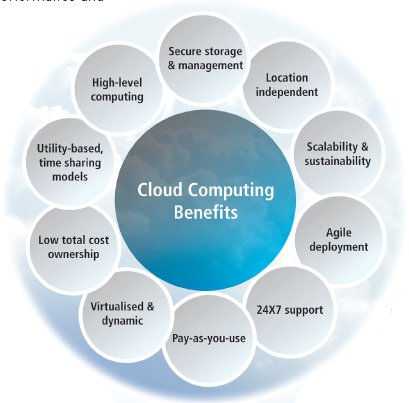
\includegraphics[scale=0.5]{imagenes/beneficiosCC.jpg}
\caption{ Beneficios Cloud Computing\cite{beneficios} }
\end{figure}


\subsection{Tipos de Nube}

Las nube puede clasificarse en distintos modelos en función del tipo de solución que quiera ofertarse:

\subsubsection{Nube Pública}

Las nubes públicas son propiedad de los proveedores de servicio, es decir, hardware, software y todos los componentes necesarios para la infraestructura virtual subyacente son propiedad del proveedor de servicio cuya tarea es administrarlos. El consumidor accede y administra los recursos que va a consumir desde un explorador web.  Algunos ejemplos de proveedores de nube pública son GoogleCloud\cite{gcp} , Amazon Web Services\cite{aws} o Microsoft Azure\cite{azure}

\subsubsection{Nube Privada}
Las nubes privadas se caracterizan por que sus servicios e infraestructura subyacente se mantiene en una red privada, utilizados exclusivamente por una empresa u organización. Por ejemplo, una nube privada puede encontrarse físicamente en el centro de datos de una compañía.

\subsubsection{Nube Híbrida}

Las nubes híbridas se caracterizan por combinar los modelos de nube pública y nube privada. La nubes híbridas inter-conectan ambos modelos con el objetivo de compartir datos y aplicaciones aportando mayor flexibilidad y opciones de desarrollo, optimizando el uso de la infraestructura subyacente y la seguridad.


\subsection{Tipos de Servicios en la Nube}

La computación en la nube permite la integración de servicios en Red dando servicio a nivel mundial y además contribuye al uso eficiente de la energía pero la centralización de las aplicaciones y el almacenamiento de los datos origina una interdependencia con los proveedores de servicios. La disponibilidad de estos servicios necesita de conexión a Internet. Los servicios que ofertados por la nube pueden clasificarse en las siguientes subsecciones:

\begin{figure}[H]
\centering
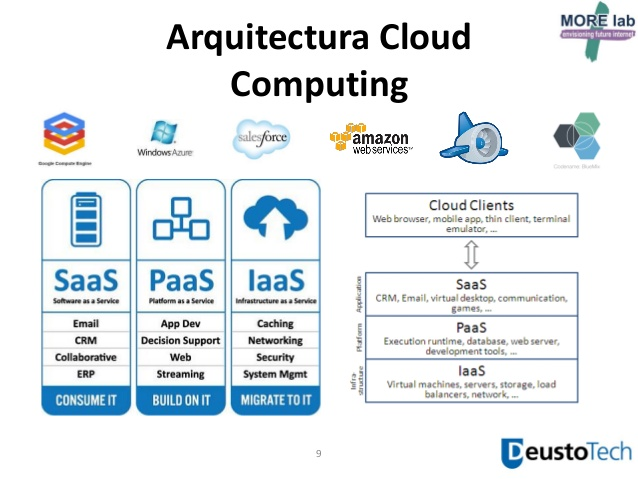
\includegraphics[scale=0.5]{imagenes/arquitecturaCC.jpg}
\caption{ Arquitectura Cloud Computing\cite{arquitecturaCC} }
\end{figure}

\subsubsection{Software como servicio (SaaS)}

El Software como Servicio\cite{saas} (SaaS, Software as a Service) ofrece el consumo de una gran variedad de aplicaciones o servicios proporcionadas por los proveedores del servicio y que se ejecutan en la infraestructura de la nube. Las aplicaciones en la nube son accesibles por distintos dispositivos del cliente a través de una interfaz sencilla, como por ejemplo un navegador web. El cliente no gestiona la infraestructura del servicio, que incluye la red de comunicaciones, los servidores, los sistemas operativos y el almacenamiento, simplemente utiliza el servicio como es el caso de este proyecto.

\subsubsection{Plataforma como servicio (PaaS)}

La Plataforma como Servicio\cite{paas} (PaaS, Platform as a Service) es una categoría de servicios cloud que proporciona un entorno a los desarrolladores crear aplicaciones y servicios que funcionen a través de internet. Los servicios PaaS se alojan en la nube, y los usuarios pueden acceder a ellos a través de un navegador web. . Los servicios PaaS consisten en funcionalidades pre-configuradas a las que los clientes puedan suscribirse, eligiendo las funciones que deseen incluir en función de sus necesidades.

Algunas de las funcionalidades PaaS son:

\begin{enumerate}
\item Sistema operativo.
\item Entorno de scripting de servidor.
\item Sistema de gestión de base de datos.
\item Software de servidor.
\item Soporte técnico.
\item Almacenamiento.
\item Acceso a la red.
\item Herramientas de diseño y desarrollo.
\item Hosting.
\end{enumerate}

\subsubsection{Infraestructura como servicio (IaaS)}

La Infraestructura como Servicio\cite{iaas} (IaaS, Infrastructure as a Service) es un servicio cloud, que proporciona acceso a recursos informáticos situados en un entorno virtualizado, a través de una conexión pública. Los recursos informáticos ofrecidos  son básicamente infraestructura de procesamiento. Físicamente, el repertorio de recursos hardware disponibles procede de multitud de servidores y redes, generalmente distribuidos entre numerosos centros de datos, de cuyo mantenimiento se encarga el proveedor del servicio cloud. El cliente, por su parte, obtiene acceso a los componentes virtualizados para construir con ellos su propia plataforma informática.

Estas son algunas de las ventajas o características de una implementación basada en el modelo de Infraestructura como Servicio:

\begin{enumerate}
\item Escalabilidad.
\item Sin necesidad de invertir en hardware.
\item Independencia de la localización.
\item Seguridad física en los centros de datos.
\end{enumerate}

\section{Programación Generativa}

Tal y como se presenta en el articulo "Generative Programming"\cite{gp} la programación generativa consiste en diseñar e implementar módulos software que pueden ser combinados para generar sistemas especializados y  optimizados en cumplir requisitos específicos de dominio. Los objetivos de la programación generativa son:

\begin{enumerate}
\item Disminuir la desviación conceptual entre el código software y los conceptos de dominio.
\item Reutilización y adaptabilidad de módulos software.
\item Simplificar la administración de muchas variantes de un componente.
\item Aumentar la eficiencia  en capacidad y en tiempo de ejecución.
\end{enumerate}


Para alcanzar estos objetivos, la programación generativa ha de cumplir los siguientes principios tratados en el articulo "Generative Programming and Active Libraries" \cite{gpl}

\begin{enumerate}
\item Separation of concerns (SoC): La separación de preocupaciones pone de manifiesto la importancia de lidiar con los problemas de una manera atómica. Es decir, crear pequeños fragmentos de código que cumplan con una funcionalidad muy especifica e integrarlos para dar lugar al componente deseado.
\item Parameterization of differences. La parametrización de componentes da la posibilidad de representar familias de componentes.
\item Analysis and modeling of dependencies and interactions. Define el termino conocimiento de configuración horizontal como la dependencia que existe en el valor que toma el parámetro de un modelo, condicionado el valor de otros parámetros del mismo modelo.
\item Separating problem space from solution space. Define el termino conocimiento de configuración vertical, donde se pone de manifiesto que el espacio del problema es especifico del dominio mientras que el espació de la solución ha de ser generalizado.
\item Eliminating overhead and performing domain-specific optimizations. Donde se aconseja un proceso de refinamiento tras la generación estática de componentes para eliminar software no utilizado en el dominio especifico.
\end{enumerate}


\section{Ciclo de Vida del Desarrollo Software (SDLC)}

El ciclo de vida del desarrollo software es un procedimiento sistemático para construir software.  El objetivo de este procedimiento es el de garantizar la calidad y las exactitud del software a desarrollar, haciendo que cumpla con las expectativas del usuario. 

Normalmente este procedimiento es aprovechado por las figuras encargadas de gestionar proyectos informáticos ya que les permite concretar el tiempo de desarrollo y los costes que supondrá la realización del mismo.   

\subsection{Etapas SDLC}


\begin{enumerate}
\item 
\item
\item
\end{enumerate}

\chapter{Problema y Solución}

En este capítulo se presenta el problema a solucionar con este proyecto. En las siguientes secciones se analizarán


Diversidad de aplicaciones cloud. Nuevas tecnologías entorno variado y cambiante. Demanda de nuevas tecnologías.
Capacitación para desarrolladores. Diversidad de aplicaciones, mismo tratamiento, simplificar proceso de aprendizaje y desarrollo software. FullStack.

\section{Definición del Problema}



 cloud  de diversa naturaleza partiendo de una especificación de alto nivel.  Normalmente, las etapas de desarrollo software están segmentadas en el desarrollo del código, la compilación de este código junto con las dependencias de terceros necesarias para producir un ejecutable, binario o artefacto para su posterior ejecución,  la configuración necesaria para poder ejecutar el artefacto resultante así como  la infraestructura virtual necesaria para desplegar y soportar la actividad de negocio de  dicho software, siendo este accesible desde Internet.


 Normalmente en los proyectos informáticos las etapas o estados que los productos software alcanzan están muy segmentadas. Descritas a muy alto nivel, estas etapas comienzan por el diseño y especificación de la solución,  continuan con el desarrollo del código fuente necesario para cumplir la solución así como las pruebas necesarias para verificar el correcto funcionamiento , la compilación de este código junto con las dependencias de terceros necesarias para producir un ejecutable, binario o artefacto para su posterior ejecución,  la configuración necesaria para poder ejecutar el artefacto resultante así como  la infraestructura virtual necesaria para desplegar y soportar la actividad de negocio de  dicho software, siendo este accesible desde Internet.




Este proyecto muestra como el uso de la programación generativa y las tecnologías de la información mejoran el proceso  aprendizaje y desarrollo software en el ámbito de las soluciones orientadas a la web 2.0.

Se pretende proporcionar al desarrollador software de un sistema web orientado a la generación, construcción y despliegue de aplicaciones web o servicios cloud  de diversa naturaleza partiendo de una especificación de alto nivel.

Normalmente, las etapas de desarrollo software están segmentadas en el desarrollo del código, la compilación de este código junto con las dependencias de terceros necesarias para producir un ejecutable, binario o artefacto para su posterior ejecución,  la configuración necesaria para poder ejecutar el artefacto resultante así como  la infraestructura virtual necesaria para desplegar y soportar la actividad de negocio de  dicho software, siendo este accesible desde Internet.

\section{Presentación de la Solución}

Para alcanzarlo, se hace uso de conceptos de programación generativa, como generalizar separar el dominio especcifico de la

en un conjunto automatizado de etapas.

 La generalización ocurre al manejar los distintos sistemas de información:

\begin{enumerate}
\item \textbf{ Aplicaciones web estáticas }
\item \textbf{ Aplicaciones web dinámicas}
\item \textbf{ Interfaces web }
\item \textbf{ Api/Rest }
\item \textbf{ Servicios }
\item \textbf{ Cualquier pieza software que pueda ser consumida mediante protocolo tcp/http }
\end{enumerate}

como una única  entidad \textbf{aplicación} y  someter a esta entidad al mismo proceso o etapas independientemente de cual sea su naturaleza o dominio cumpliendo con el objetivo de dada una especificación de aplicación, producir el código y/o configuración necesaria para materializar dicha especificación en un producto software, construir un artefacto auto-contenido que permita la ejecución del software generado, ejecutar dicho artefacto sobre la infraestructura virtual necesaria para que la aplicación especificada sea accesible por Internet y que de esta forma el usuario de este proyecto sea capaz de consumir la aplicación generada.

\chapter{Planificación y Análisis}


Con el objetivo de generalizar y definir aplicación software se han decidido usar las partes:

Repositorio
Readme
Makefile
Licencia
src codigo fuente
config configuración


\begin{enumerate}
\item \textbf{ Code Generation }  Etapa inicial donde se sintetiza el proceso de desarrollo software, es decir se produce el código necesario para la solución especificada por el desarrollador.
\item \textbf{ Artefact Generation }  El objetivo de esta etapa es aprovechar el código fuente generado en la etapa Code Generation para producir un artefacto auto-contenido junto con la configuración necesaria para su ejecución en un entorno virtual.
\item \textbf{ Deploy Generation } En esta etapa se aprovecha el producto de la etapa Artefact Generation para disponibilizar la solución en Internet.
\end{enumerate}


Programación generativa: generar, automatizar  y despliegue accesible a Internet.


La aplicación software es el elemento de negocio de este sistema.  Para materializar esto, el sistema crea un repositorio de código por cada aplicación creada para albergar la producción de código especificado por  el desarrolador.


Generar: Aplicaciones completas, independientemente de la tecnología, utilidad o fin. Las aplicaciones generadas por el sistema
son auto-contenidas y automatizadas, es decir mantienen una semántica común




d
test
run
pull
push

Lo que permite al desarrollador integrar fácilmente nuevos cambios.

Definir el permino produción dentro del marco de este sistema, consiste en la siguiente serie de etapas:

\section{Planificación}

La planificación temporal muestra mediante el uso de diagramas de Gant la distribución en el tiempo de las tareas necesarias para cumplir con los objetivos de esta proyecto.

--  TODO -- INCLUIR DIAGRAMAS GANT


\section{Análisis Software}

El análisis software pone de manifiesto la especificación del sistema software a construir. Dirigida por Ingeniería de requisitos y de casos de uso, las siguientes subseciones muestran las partes y funcionalidades que el sistema resultante ha de cumplir.

\subsection{Requisitos de Información }
Los requisitos de información se caracterizan por reunir la información relevante para la solución, que debe gestionar y almacenar el sistema software.\\

\textbf{RI-1. Workspace:} Representación del espacio de trabajo del usuario. Contiene el conjunto de las aplicaciones que el usuario ha creado usando el sistema. Concepto similar al del Escritorio o "Desktop" de un sistema operativo.
Contenido: nombre de usuario o propietario del workspace, referencia al conjunto de aplicaciones generadas.


\textbf{RI-2. App:} Representación de cada una de las aplicaciones generadas por el sistema.
Contenido:
\begin{lstlisting}[language=json,firstnumber=1]
{
    "_id" : "appName",
    "repo" : "https://github.com/user/appName.git",
    "spec" : {
        "dockerId" : "appNameDockerId",
        "port" : "4343",
        "nature" : "staticApp"
    },
    "des" : "",
    "url" : "http://deploy.domain:4343",
    "owner" : "user>s",
    "status" : "running"
}
\end{lstlisting}

\textbf{RI-3. Información de Usuario:} Información sensible del usuario o desarrollador que va a usar el sistema. Credenciales al sistema de gestión de repositorios para el código fuente, en este caso relativa al perfil de github.
Contenido: nombre de usuario, correo electrónico, organización. \\


\subsection{Requisitos Funcionales }
Como se define en la ingeniería de requisitos, los requisitos funcionales establecen el comportamientos del sistema.\\



\subsubsection { \textbf{ RF-1. Gestión de aplicaciones.}} El sistema ha de gestionar el ciclo de vida de las aplicaciones generadas.\\

\textbf{RF-1.1.} El sistema permitirá crear aplicaciones.
\begin{itemize}
 \item 	\textbf{RF-1.1.1.}El sistema generará aplicaciones de diversa naturaleza, tecnología o dominio. Añadir referencia a especificación de aplicaciones.
 \item 	\textbf{RF-1.1.2.}El sistema creará y  guardará en repositorios de código las aplicaciones generadas.
  \item \textbf{RF-1.1.3.}El sistema construirá los artefactos necesarios para ejecutar las aplicaciones generadas.
   \item  \textbf{RF-1.1.4.} El sistema ejecutará los artefactos construidos para disponibilizar vía Internet las aplicaciones creadas. \\
\end{itemize}


\textbf{RF-1.2.} El sistema permitirá eliminar aplicaciones.
\begin{itemize}
 \item 	\textbf{RF-1.2.1.}El sistema detendrá los artefactos en ejecución de aplicaciones eliminadas.
  \item 	\textbf{RF-1.2.2.}El sistema eliminará los artefactos construidos de aplicaciones eliminadas.
   \item  \textbf{RF-1.2.3.}El sistema eliminará los repositorios de código de aplicaciones eliminadas.	\\
\end{itemize}


\textbf{RF-1.3.} El sistema permitirá ejecutar aplicaciones.
\begin{itemize}
 \item \textbf{RF-1.3.1.} El sistema será capaz de hacer a las aplicaciones accesibles vía Internet.
 \item  \textbf{RF-1.3.2.} El sistema proporcionará las herramientas  y configuraciones necesarias para que las aplicaciones puedan ser ejecutas en local y ser accesibles vía \textbf{localhost}  \\
\end{itemize}


\textbf{RF-1.4.} El sistema permitirá detener aplicaciones.

\begin{itemize}
 \item  \textbf{RF-1.4.1.} El sistema será capaz de detener las aplicaciones que sean accesibles vía Internet.
  \item  \textbf{RF-1.4.2.} El sistema deberá liberar los recursos virtuales correspondientes a la aplicación detenida.
  \item  \textbf{RF-1.4.3.} El sistema proporcionará las herramientas  y configuraciones necesarias para que las aplicaciones ejecutadas en \textbf{localhost}  sean detenidas de manera controlada. \\
\end{itemize}

\textbf{RF-1.5.} El sistema permitirá visualizar información de las aplicaciones.

\begin{itemize}
\item \textbf{RF-1.5.1.} El sistema permitirá consultar  información de utilidad relativa a las aplicaciones,  como por ejemplo, especificación, URL del repositorio donde se alberga el código fuente, URL o IP donde la aplicación puede ser consumida vía Internet.
\item \textbf{RF-1.5.2.} El sistema permitirá inspeccionar aplicaciones. El sistema permitirá a los usuario consultar información de DEBUG de las aplicaciones accesibles vía Internet, es decir, permitirá consultar LOGs de aplicaciones en ejecución.
\item \textbf{RF-1.5.3.} El sistema permitirá visualizar información del estado del ciclo de vida de las aplicaciones. El ciclo de vida de las aplicaciones del sistema se representará con el siguiente flujo de estados:\\
\end{itemize}


\subsubsection { \textbf{ RF-2. Gestión de credenciales.}} El sistema proporcionará los mecanismos necesarios para que los usuarios se autentiquen en el sistema. \\


\textbf{RF-2.1.} El sistema  permitirá iniciar sesión  a los usuarios mediante nombre de usuario y contraseña. Típicamente estas credenciales corresponderán al sistema de gestión de repositorios de código.

\textbf{RF-2.3.} El sistema  permitirá cerrar sesión a los usuarios de manera controlada, es decir, mantendrá las aplicaciones en ejecución.

\textbf{RF-2.3.} El sistema  realizará todas las operaciones que requieran autenticación mediante TOKEN.

\textbf{RF-2.4.} El sistema  proporcionará a los usuarios el TOKEN necesario para trabajar localmente con las aplicaciones.


\subsection{Requisitos No Funcionales }
Los requisitos no funcionales, se refieren a todos los requisitos que no describen información a guardar, ni funciones a realizar por el sistema, sino características de funcionamiento.\\


\textbf{RNF-1} Se necesitará acceso a Internet para utilizar las funcionalidades del sistema.\\

\textbf{RNF-2} Se necesitará una cuenta en Github para utilizar las funcionalidades del sistema.\\

\textbf{RNF-3} Se prestará especial atención en la gestión de credenciales de los usuarios.\\

\textbf{RNF-4} Se prestará especial atención en la seguridad del  las aplicaciones expuestas a Internet.
\subsection{Casos de Uso}
Los diagramas de casos de uso, son diagramas UML que representan gráficamente a todos los elementos que forman parte del modelo de casos de uso junto con la frontera del sistema. Delimitan el sistema a diseñar. Determinan el contexto del uso del sistema. Describen el punto de vista de los usuarios  en el sistema.


\begin{figure}[H]
\centering
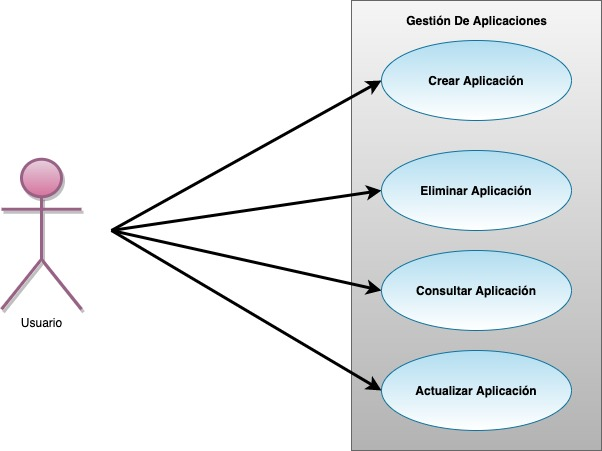
\includegraphics[scale=0.50]{imagenes/casosUso1.jpg}
\caption{ Casos de uso - Gestión Aplicaciones I\cite{diagrama}  }
\end{figure}

\begin{figure}[H]
\centering
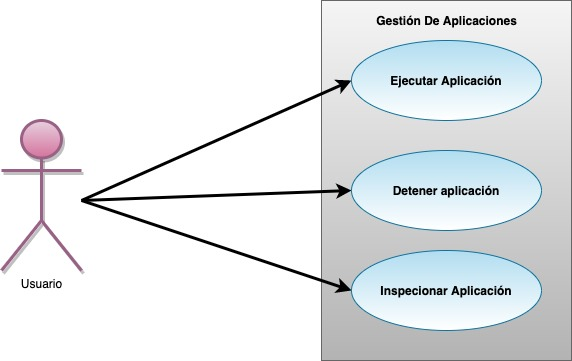
\includegraphics[scale=0.50]{imagenes/casosUso2.jpg}
\caption{ Casos de uso - Gestión Aplicaciones II\cite{diagrama}  }
\end{figure}

\begin{figure}[H]
\centering
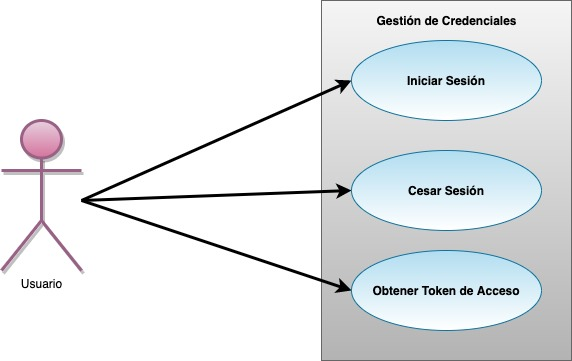
\includegraphics[scale=0.50]{imagenes/casosUso3.jpg}
\caption{ Casos de uso - Gestión Credenciales\cite{diagrama}  }
\end{figure}

\subsection{Diagramas de Secuencia}
Los diagramas de secuencia especifican las interacciones temporales entre las piezas internas del sistema para cumplir con las funcionalidades requeridas.


\begin{figure}[H]
\centering
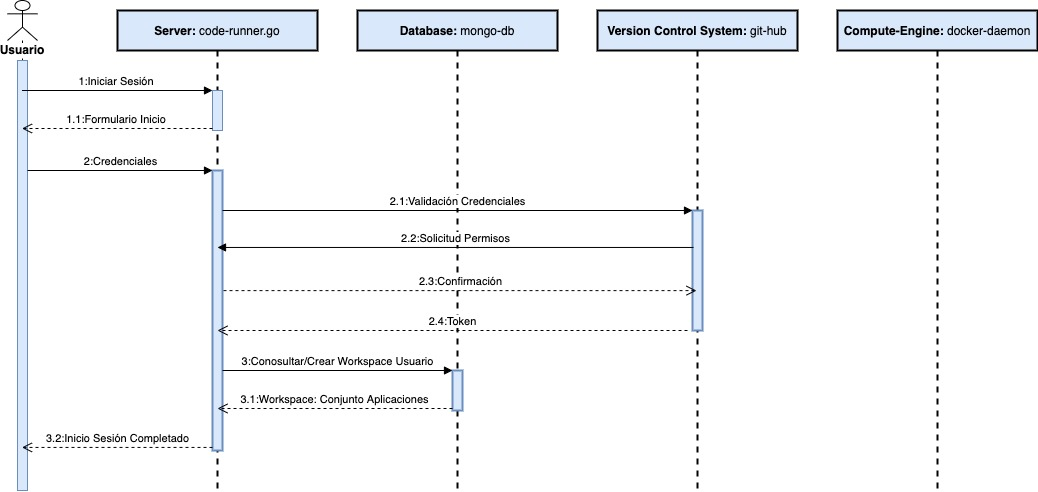
\includegraphics[scale=0.45]{imagenes/secuencia1.jpg}
\caption{ Diagramas de Secuencia - Inicio sesión \cite{diagrama}  }
\end{figure}

\begin{figure}[H]
\centering
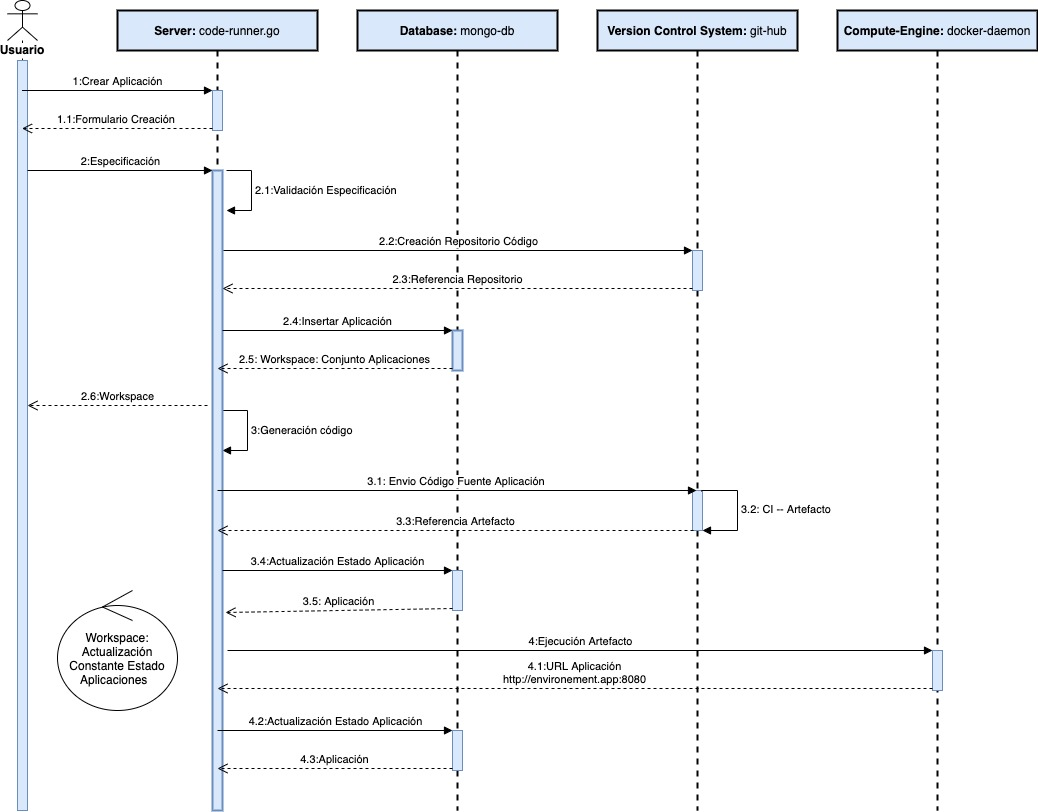
\includegraphics[scale=0.43]{imagenes/secuencia2.jpg}
\caption{ Diagramas de Secuencia - Crear Aplicación\cite{diagrama}  }
\end{figure}


\begin{figure}[H]
\centering
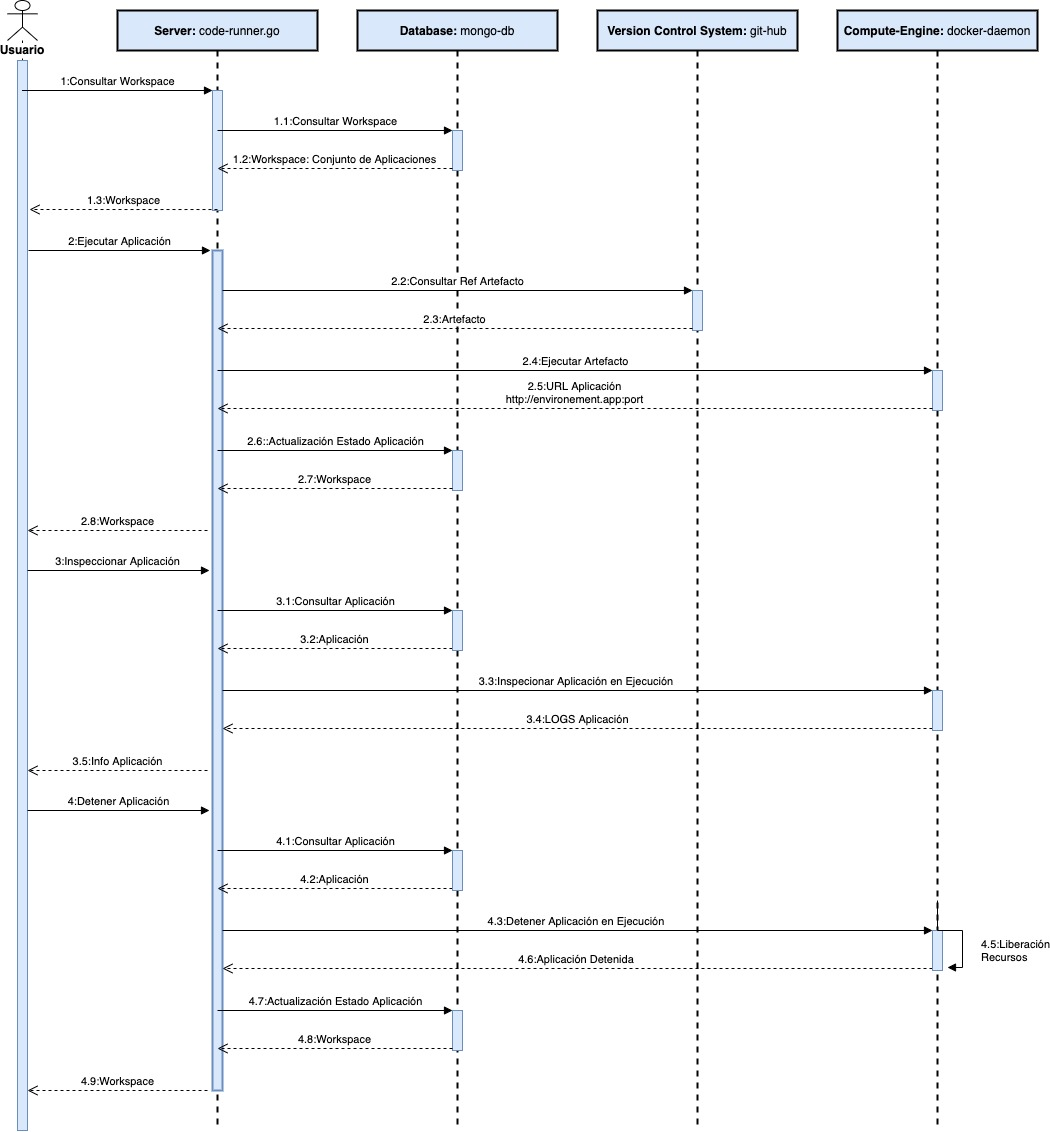
\includegraphics[scale=0.43]{imagenes/secuencia3.jpg}
\caption{ Diagramas de Secuencia - Ejecutar, Inspeccionar y Detener Aplicación\cite{diagrama}  }
\end{figure}

\begin{figure}[H]
\centering
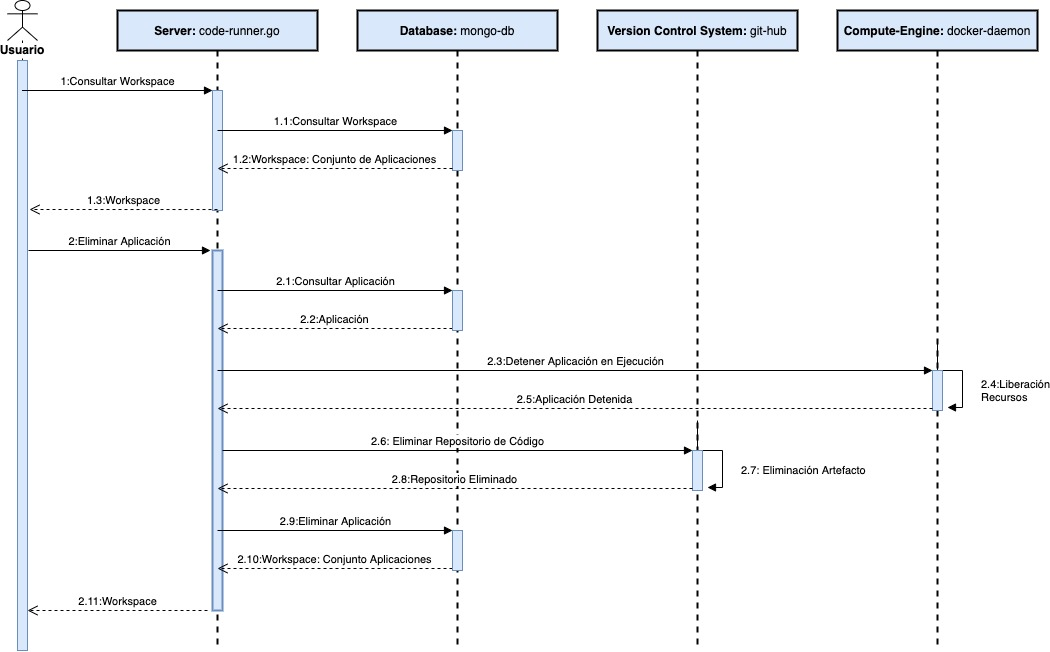
\includegraphics[scale=0.43]{imagenes/secuencia4.jpg}
\caption{ Diagramas de Secuencia - Eliminar Aplicación\cite{diagrama}  }
\end{figure}





\chapter{ Implementación y Pruebas}


\section{Desarrollo}

En el proceso de desarrollo del sistema, se ha seguido el patrón de arquitectura software modelo-vista-controlador (MVC)\cite{mvc} cuya finalidad es separar los datos y la lógica de una aplicación de la interfaz de usuario. Este patrón de arquitectura se basa en la re-utilización de código y separación de conceptos. El objetivo de esta metodología es el de facilitar el desarrollo, mantenimiento y esca-labilidad del software resultante.

\begin{figure}[H]
\centering
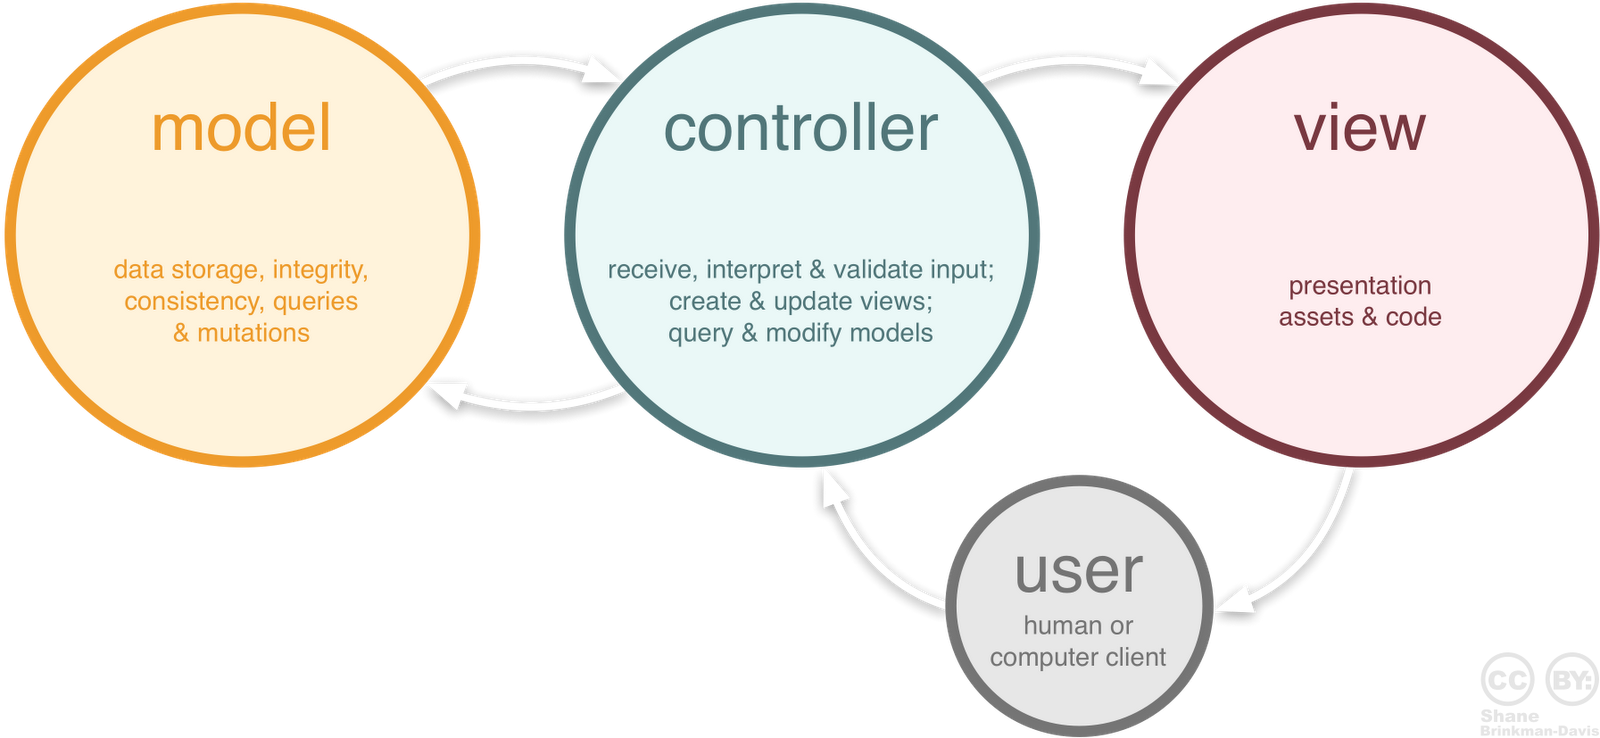
\includegraphics[scale=0.20]{imagenes/mvc.png}
\caption{ Modelo-Vista-Controlador\cite{mvc2}  }
\end{figure}

Los componentes\cite{mvc3}\cite{mvc4} del Modelo-Vista-Controlador se pueden definir en:

\begin{enumerate}
\item \textbf{Modelo:} Representa la información , gestionando los accesos a ella, la base de datos  o capa de persistencia es un componente del modelo.

\item \textbf{Vista:} Representa el modelo en un formato adecuado para interactuar con él mediante la interfaz de usuario.

\item \textbf{Controlador:} Responde a eventos invocando peticiones al modelo cuando se hace alguna solicitud de la información (por ejemplo, editar un documento o un registro en una base de datos). El controlador interactúa con su vista asociada para realizar cambios en la forma de representar el modelo.
\end{enumerate}


Como parte del desarrollo del proyecto también se ha utilizado la metodología de ingeniería del software conocida como desarrollo basado en test o TDD. Dicha metodología consiste en escribir los test necesarios para cubrir las funcionalidades del sistema y a partir de ellos, escribir el código necesario para que dichas pruebas sean superadas, cumpliendo así la funcionalidad que se esta poniendo a prueba.  En las siguientes subsecciones se detallarán las partes que forman el sistema así como las tecnologías utilizadas para su desarrollo.

\subsection{Back-End}

El Back-End o servidor se refiere a la parte trasera del sistema, donde ocurre toda la lógica y funcionalidad pero que es transparente para el usuario final que consume el sistema. Para facilitar la comprensión de las partes que forman  el back-end del proyecto se van a desglosar en las siguientes subsecciones.

\subsubsection{Servidor}

El servidor es la entidad principal del Back-End, contiene la lógica del sistema y es el responsable de la comunicación entre el resto de partes del back-end y de servir o renderizar las vistas al cliente.
El servidor ha sido desarrollado utilizando Golang\cite{go} como lenguaje de programación. Inicialmente se pensó en utilizar Javascript bajo el framework NodeJS, ya que dicho marco de trabajo funciona de manera asíncrona, lo que facilita muchas de las operaciones en segundo plano que este sistema ha de realizar, ademas NodeJS facilita la integración del servidor con diversas tecnologías cliente basadas también en Javascript. Una de las principales deficiencias  observadas en el uso de Javascript para el desarrollo del servidor de este proyecto es el menejo de templates o plantillas.
En la etapa de generación de código la templatización de los modelos de datos necesarios para producir aplicaciones es vital, no solo en su implementación si no también en la eficiencia de estas operaciones y es aquí donde Golang destaca, ya que permite serializar estructuras de datos complejas y utilizar dicha representación para crear contenido. Otra ventaja que proporciona utilizar Golang en este proyecto es el uso de Go-Routinas, es decir, la capacidad de ejecutar funcionalidad en segundo plano de una manera sencilla y controlada junto con la generalizacióon de la implementación mediante interfaces hacen que Golang sea el lenguaje de programación adeacuado para el desarrollo de este proyecto.  Es interesante destacar que Golang ha sido diseñado para optimizar el uso concurrente de las aplicaciones creadas con él, lo que mejora considerablemente los tiempos de respuesta y la experiencia de usuario.

\subsubsection{Persistencia de Datos}

La parte imprescindible para la capa de acceso a datos es el sistema gestor de bases de datos, encargado de almacenar los modelos del sistema. Como propuesta inicial para el desarrollo del sistema, se pensó en utilizar un esquema relacional utilizando sistemas gestores de bases de datos relacionales como MySQL o PostgreSQL  por la facilidad de diseño entidad-relación.

La principal desventaja de modelar el problema mediante entidad-relación es la perdida en la flexibilidad de los modelos de datos ya que este esquema tradicional obliga a que todas las filas de una tabla representativa de un modelo tengan los mismos campos para mantener la entidad referencial y debido a la diversidad de aplicaciones que este sistema es capaz de manejar se requiere que el modelo de datos sea flexible. Debido a esto, se ha decido utilizar MongoDB\cite{mg} como sistema gestor de bases de datos no-relaciones también denominadas bases de datos documentales, con el objetivo de conseguir un esquema interno flexible y eficiente.

\begin{figure}[H]
\centering
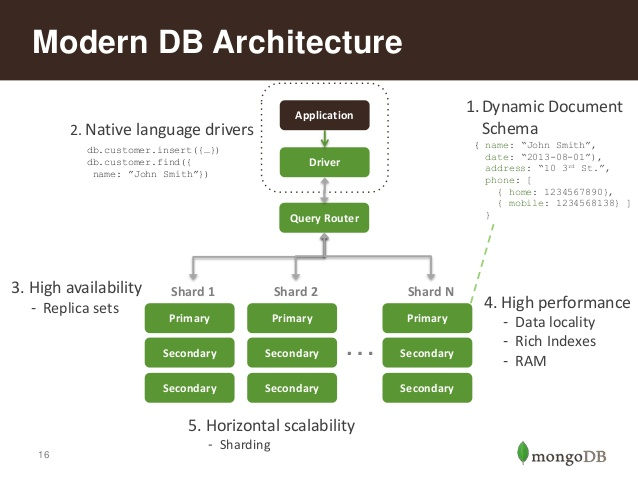
\includegraphics[scale=0.30]{imagenes/mongo.jpg}
\caption{ Arquitectura MongoDB\cite{mongoA}  }
\end{figure}

MongoDB es un sistema de base de datos NoSQL orientado a grandes cantidades de datos, guarda estructuras de datos en documentos similares a JSON. Se trata de una base de datos ágil que permite cambiar los esquemas de una aplicación cuando esta evoluciona. Los principales objetivos de estas bases de datos son la escalabilidad, rendimiento y gran disponibilidad.

En MongoDB los documentos se agrupan en colecciones. Las colecciones  no imponen una estructura fija a los documentos que contienen, ni siquiera al tipo de datos de cada campo. Esto es una ventaja cuando las entradas de la base de datos dependen de la naturaleza de las aplicaciones que el usuario final quiera generar.


\subsubsection{Repositorio de Código}

Las entidades generadas por este sistema ( aplicaciones) están compuestas por un conjunto de ficheros ( README, licencia, código fuente, configuración, scripts, makefile, dockerfile...etc), estos ficheros producidos por el sistema son almacenados en repositorios de código alojados en la nube de manera pública, para ello, este proyecto esta completamente integrado con Github\cite{github}.

GitHub\cite{github} es una plataforma de desarrollo colaborativo de software para alojar proyectos utilizando el sistema de control de versiones Git. El código es almacenado de forma pública o privada. GitHub aloja el código en repositorios y brinda herramientas muy útiles para trabajar de forma colaborativa. Github\cite{github2} ofrece varias herramientas:

\begin{enumerate}
\item Una wiki para el mantenimiento de las distintas versiones de las aplicaciones.
\item Un sistema de seguimiento de problemas que permiten a los miembros de un equipo de desarrollo detallar problemas software.
\item Una herramienta de revisión de código, donde se pueden añadir anotaciones en cualquier punto de un fichero y debatir sobre determinados cambios realizados en un commit específico.
\item Un visor de ramas donde se pueden comparar los progresos realizados en las distintas ramas de un repositorio.
\end{enumerate}


Este proyecto aprovecha principalmente las siguientes funcionalidades ofertadas por Github:

\begin{enumerate}
\item \textbf{ Autenticación.} El usuario final que utilice este sistema para generar aplicaciones necesita una cuenta de github, ya que la autenticación mediante user/pass corresponde con el user/pass de su cuenta de github. Esto permite al sistema crear repositorios y pushear código a dichos repositorios bajo el perfil del usuario registrado. El proceso de autenticación contra Github proporciona una accesToken el cual es aprovechado por los usuarios del sistema para trabajar localmente con las aplicaciones generadas por el sistema.

\item   \textbf{Integración Continua.} Github proporciona las denominadas GitHub-Actions\cite{github3}  que permiten automatizar, customizar y ejecutar flujos de integración continua  sobre los proyectos software alojados en sus repositorios, para ello, en el proceso de Code Generatión este sistema produce un fichero  en el path  <repositorio>/.github/workflows/ci.yml donde se generaliza el proceso de compilación, testing y empaquetado del la aplicación contenida en el repositorio, independientemente de la naturaleza de la aplicacióno, dando lugar a un artefacto auto-contenido listo para ser desplegado sobre un entorno virtual. Los artefactos generados son Imágenes Docker las cuales se veran en mas detalle en la siguiente sub-sección.

\item \textbf{Gestión de Artefactos} Github proporciona los denominados GitHub-Packages\cite{github4} que permiten publicar y consumir paquetes o artefactos resultado de la compilación y empaquetado de las aplicaciones software albergadas en un repositorio de código. GitHub-Packages es capaz de gestionar paquetes de diversa naturaleza, siendo las imágenes docker las utilizadas en este proyecto.
\end{enumerate}

\subsubsection{Infraestructura Virtual de las Aplicaciones}

La infraestructura virtual de las aplicaciones  representa al entorno de computación en la nube que cuenta con los recursos necesarios para ejecutar o desplegar las aplicaciones generadas por el proyecto, permitiendo a los usuarios utilizar las aplicaciones generadas vía Internet.
Con el objetivo de generalizar la gestión de aplicaciones  se ha decidido utilizar Docker como tecnología de virtualización ligera.

Docker\cite{dk} es una herramienta para automatizar el despliegue de aplicaciones dentro de contenedores, proporcionando una capa de abstracción y automatización de virtualización a nivel de sistema operativo. Docker utiliza aislamiento de recursos del kernel de Linux, para permitir que contenedores independientes se ejecuten dentro de una sola máquina, evitando la sobrecarga de iniciar y mantener máquinas virtuales.

\begin{figure}[H]
\centering

\includegraphics[scale=0.35]{imagenes/docker.png}
\caption{ Virtualización Docker\cite{dkw}}
\end{figure}

La principal diferencia con respecto a máquinas virtuales es el tamaño. Las máquinas virtuales incluyen la aplicación, el código, las librerías necesarias y un sistema operativo anfitrión completo mientras que los contenedores contienen lo mismo pero comparten el núcleo con otros contenedores corriendo como un proceso asilado en el espacio de usuario del sistema operativo anfitrión. No están vinculados con ninguna infraestructura especifica.

Docker aporta a este proyecto la capacidad de abstraer las aplicaciones de la infraestructura virtual subyacente. En la etapa de Code Generation se produce un fichero denominado Dockerfile con la definición necesaria para ejecutar la aplicación producida en un contenedor. Este fichero es aprovechado  por el flujo de integración continua definido en (incluir referencia a ci.yml)  para producir una imagen docke como artefacto. Este artefacto es utilizado para crear un contenedor docker en un entorno virtual acesible a internet, habilitando el puerto necesario para garantizar que el trafico es redireccionado al contenedor adecuado.


\subsection{Front-end}

El Front-End, capa de presentación o capa de cliente es la encargada de controlar la interacción con el usuario. En este proyecto la programación en el lado cliente para mantener  información actualizada del estado en el que se encuentran las aplicaciones producidas por el sistema. Para ello, se aprovecha el motor de plantillas proporcionado por el servidor GO junto con JQuery y Ajax para realizar llamadas asíncronas al servidor y actualizar dinámicamente los datos que percibe el cliente.

\subsubsection{Tecnología Cliente}


JQuery\cite{jq} es una librería de JavaScript, que permite interactuar con los documentos HTML, manipular el árbol DOM, manejar eventos, desarrollar animaciones y agregar interacción con el servidor mediante llamadas asíncronas realizadas con Ajax. Su objetivo principal es dar un comportamiento dinámico a la web. Jquery funciona en múltiples navegadores y es compatible con CSS3.

Ajax\cite{aj}, abreviatura de JavaScript Asíncrono y XML es un conjunto de técnicas de desarrollo web en el cliente para crear aplicaciones asíncronas y dinámicas. Con Ajax, las aplicaciones pueden enviar y recibir datos desde el servidor en segundo plano sin que interfiera en la visualización o el comportamiento de la aplicación. Utilizar Ajax supone crear aplicaciones web en las que la capa de intercambio de datos ha sido separada de la capa de presentación, lo que permite un comportamiento dinámico sin la necesidad de recargar el navegador.


Socket  --> Logs aplicaciones en tiempo real.

\subsection{Infraestructura Virtual}
Heroku ( plataforma as a service) para ejecutar code-runner.go + Maquina expuesta a internet en google cloud ccon un demonio docker expuesto por el puerto 5555 comunicada con el servidor mediant TLS.

\subsection{Seguridad}

mutual tls

\chapter{Conclusiones}


\section{Mejoras}

\section{Trabajos Futuros}




\begin{thebibliography}{}

%cloud computing
\bibitem[]{RAI} \textsc{Real Academia de Ingeniería},
\textit{Acepciones}
\url{http://diccionario.raing.es/es/lema/computaci\%C3\%B3n-en-la-nube}


\bibitem[]{magazine} \textsc{Magazine Communications of the ACM },
\textit{A view of cloud computing}
\url{http://dl.acm.org/citation.cfm?doid=1721654.1721672}

\bibitem[]{gcp} \textsc{Google Cloud Platform},
\textit{Google Cloud Platform: Crea, moderniza y escala tu negocio}
\url{https://cloud.google.com}

\bibitem[]{aws} \textsc{Amazon Web Services},
\textit{Amazon Web Services: Plataforma Cloud Pública}
\url{https://aws.amazon.com}

\bibitem[]{azure} \textsc{Microsoft Azure},
\textit{Microsoft Azure: Convierta las ideas en soluciones con más de 100 servicios para crear, implementar y administrar aplicaciones}
\url{https://azure.microsoft.com}


\bibitem[]{beneficios} \textsc{Cloud Computing},
\textit{Imagen de CLOUD COMPUTING HOY - Mario josé Villamizar Cano}
\url{https://es.slideshare.net/mariojosevillamizarcano/cloud-computing-hoy-todo-como-servicio}

\bibitem[]{arquitecturaCC} \textsc{Cloud Computing},
\textit{Imagen Arquitectura}
\url{http://image.slidesharecdn.com/tocandolanubev2-141007052808-conversion-gate01/95/cloud-computing-una-perspectiva-tecnolgica-9-638.jpg?cb=1412659848}


\bibitem[]{saas} \textsc{SaaS},
\textit{¿Qué es SaaS? Software como servicio}
\url{https://azure.microsoft.com/es-es/overview/what-is-saas/}

\bibitem[]{paas} \textsc{PaaS},
\textit{What Is Platform-as-a-Service?}
\url{https://www.cloudflare.com/learning/serverless/glossary/platform-as-a-service-paas}

\bibitem[]{iaas} \textsc{IaaS},
\textit{¿Qué es IaaS? Infraestructura como servicio}
\url{https://azure.microsoft.com/es-es/overview/what-is-iaas/}

%GP

\bibitem[]{gp} \textsc{Generative Programming},
\textit{Czarnecki, Krzysztof \&  Østerbye, Kasper \& Völter, Markus. (2002). Generative Programming.}
\url{https://www.researchgate.net/publication/220842465_Generative_Programming}


\bibitem[]{gpl} \textsc{Generative Programming and Active Libraries},
\textit{K. Czarnecki, U. Eisenecker, R. Glück, D. Vandevoorde, and T. Veldhuizen. GenerativeProgramming and Active libraries.}
\url{https://pdfs.semanticscholar.org/8605/bec5fce4e8428fcb720ff07eccbeb147e9fc.pdf}

%Analisis
\bibitem[]{diagrama} \textsc{Diagrama},
\textit{Diagrama Elaboración Propia - Draw.io}
\url{https://www.draw.io}

\bibitem[]{mvc} \textsc{MVC},
\textit{MVC: Patrón de arquitectura de software }
\url{http://librosweb.es/libro/jobeet_1_4/capitulo_4/la_arquitectura_mvc.html}

\bibitem[]{mvc2} \textsc{MVC},
\textit{MVC: Diagrama}
\url{https://yalantis.com/media/content/ckeditor/2014/05/mvc_role_diagram.png}

\bibitem[]{mvc3} \textsc{MVC},
\textit{MVC: Componentes}
\url{http://martinfowler.com/eaaDev/uiArchs.html}

\bibitem[]{mvc4} \textsc{MVC},
\textit{MVC Wikipedia}
\url{https://es.wikipedia.org/wiki/Modelo%E2%80%93vista%E2%80%93controlador}


%Desarrollo
\bibitem[]{go} \textsc{Golang},
\textit{Golang}
\url{https://golang.org}

\bibitem[]{mg} \textsc{mongo},
\textit{MongoDB}
\url{https://www.mongodb.com/}

\bibitem[]{mongoA} \textsc{MongoDB},
\textit{Arquitectura MongoDB}
\url{http://image.slidesharecdn.com/enterprisearchitectsview2014-oct-141029130130-conversion-gate01/95/an-enterprise-architects-view-of-mongodb-16-638.jpg?cb=1414587854}


\bibitem[]{github} \textsc{GitHub},
\textit{How people build software}
\url{https://github.com/}


\bibitem[]{github2} \textsc{Conociendo GitHub},
\textit{readthedocs.io }
\url{http://conociendogithub.readthedocs.io/en/latest/data/introduccion/#que-es-github}

\bibitem[]{github3} \textsc{GitHub Actions},
\textit{Documentación de GitHub Actions }
\url{https://help.github.com/es/actions}


\bibitem[]{github4} \textsc{GitHub Packages},
\textit{Documentación de GitHub Packages }
\url{https://github.com/features/packages}

\bibitem[]{dk} \textsc{Docker},
\textit{Docker - Aislamiento de recursos}
\url{https://www.docker.com/what-docker}

\bibitem[56]{dkw} \textsc{Docker-Wiki},
\textit{Docker - Wikipedia}
\url{https://es.wikipedia.org/wiki/Docker_\%28software\%29}


\bibitem[]{jq} \textsc{JQuery},
\textit{JQuery Oficial}
\url{https://jquery.com/}


\bibitem[]{aj} \textsc{Ajax},
\textit{Ajax: Libros Web}
\url{https://librosweb.es/libro/ajax/}


\end{thebibliography}

\chapter{ Anexo}



%
%
%%\nocite{*}
%\bibliography{bibliografia/bibliografia}\addcontentsline{toc}{chapter}{Bibliografía}
%\bibliographystyle{miunsrturl}
%
%\appendix

%\input{apendices/manual_usuario/manual_usuario}
%%\input{apendices/paper/paper}
%\input{glosario/entradas_glosario}
% \addcontentsline{toc}{chapter}{Glosario}
% \printglossary

\thispagestyle{empty}

\end{document}
